\documentclass[tikz,border=2pt]{standalone}
\usepackage{amsmath,amssymb}
\usepackage{tikz}
\usetikzlibrary{arrows.meta}

\begin{document}
% Two equality constraints meeting at x*: with independent gradients (rank 2) the feasible set
% is a genuine point and multipliers exist; with tangent constraints (rank 1) the gradients
% are parallel, the qualification fails, and the Lagrange conditions may give no multipliers.
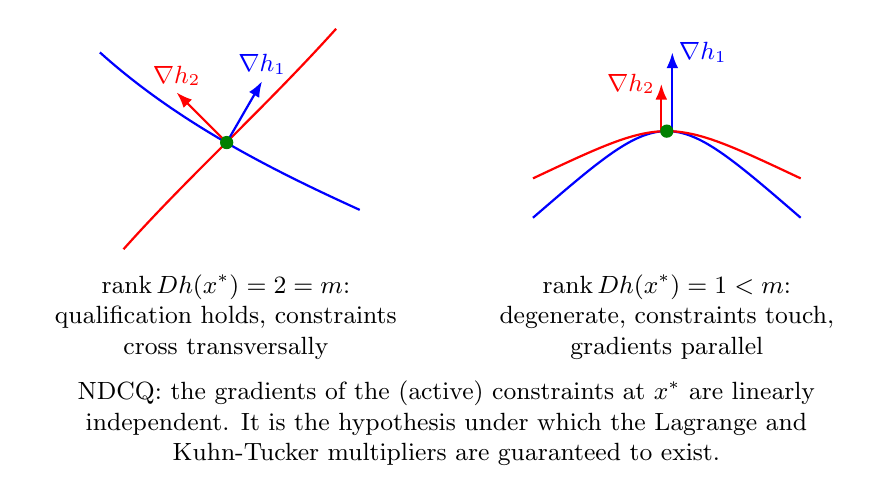
\begin{tikzpicture}[every node/.style={font=\small}, >={Latex[length=2mm]}]
	\begin{scope}
		\draw[blue, thick] (-0.4,2.5) .. controls (0.6,1.6) and (1.8,1.0) .. (2.9,0.5);
		\draw[red, thick] (-0.1,0.0) .. controls (0.7,0.9) and (1.7,1.8) .. (2.6,2.8);
		\draw[->, blue, thick] (1.21,1.355) -- (1.66,2.134) node[above, inner sep=2pt] {$\nabla h_1$};
		\draw[->, red, thick] (1.21,1.355) -- (0.574,1.991) node[above, inner sep=2pt] {$\nabla h_2$};
		\fill[green!50!black] (1.21,1.355) circle (2.4pt);
		\node[anchor=north, align=flush center, text width=4.8cm] at (1.2,-0.2) {$\operatorname{rank}Dh(x^\ast)=2=m$: qualification holds, constraints cross transversally};
	\end{scope}
	\begin{scope}[xshift=5.6cm]
		\draw[blue, thick] (-0.5,0.4) .. controls (1.2,1.867) .. (2.9,0.4);
		\draw[red, thick] (-0.5,0.9) .. controls (1.2,1.7) .. (2.9,0.9);
		\draw[->, blue, thick] (1.27,1.5) -- (1.27,2.5) node[right, inner sep=2pt] {$\nabla h_1$};
		\draw[->, red, thick] (1.13,1.5) -- (1.13,2.1) node[left, inner sep=2pt] {$\nabla h_2$};
		\fill[green!50!black] (1.2,1.5) circle (2.4pt);
		\node[anchor=north, align=flush center, text width=4.8cm] at (1.2,-0.2) {$\operatorname{rank}Dh(x^\ast)=1<m$: degenerate, constraints touch, gradients parallel};
	\end{scope}
	\node[anchor=north, align=flush center, text width=10cm] at (4.0,-1.55) {NDCQ: the gradients of the (active) constraints at $x^\ast$ are linearly independent. It is the hypothesis under which the Lagrange and Kuhn-Tucker multipliers are guaranteed to exist.};
\end{tikzpicture}
\end{document}
